\documentclass{beamer} 
\usepackage[utf8]{inputenc}
\usepackage{graphicx}
\usepackage{array, boldline, makecell, booktabs}
\newcommand\btrule[1]{\specialrule{#1}{0pt}{0pt}}
 
\title[About Beamer]
{Polyphase Filter Banks:  A Physicist's Understanding}
%Information to be included in the title page:
\author{Matthew B. Cooper}
\institute{New Jersey Institute of Technology}
\date{May 8th, 2019}
\begin{document}
 
\frame{\titlepage}
 
\begin{frame}
\frametitle{Introduction}
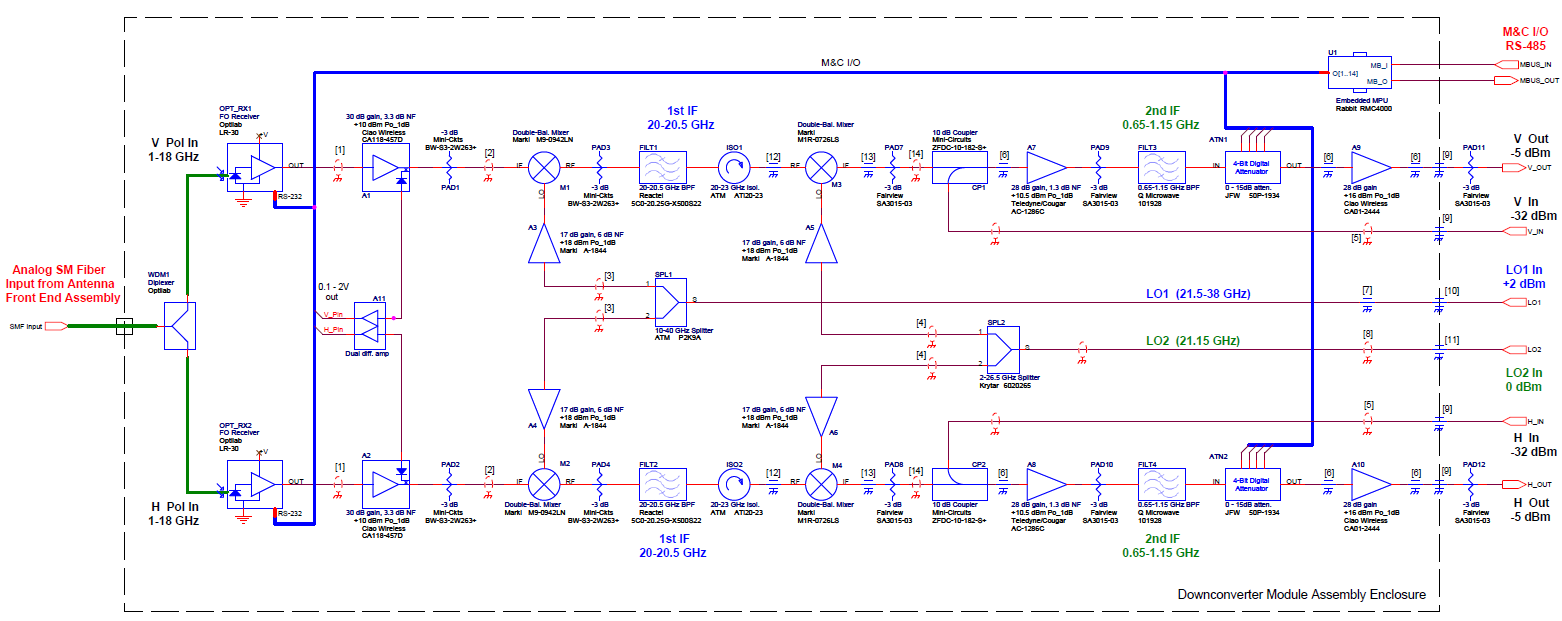
\includegraphics[scale=.25]{Figure_1.png}\footnotemark

\smallskip
The digital revolution has changed many aspects of modern life.  Scientific instrumentation has been no exception.  
\footnotetext[1]{$https://web.njit.edu/gary/728/assets/EOVSA\_DCM.PNG$}
\end{frame}

\begin{frame}
\frametitle{Et Tu, Science? And So Falls Analog.}
In most modern arrays, the signal is digitized at the receiver, then sent to the control room.  Why? 
\end{frame}

\begin{frame}
\frametitle{Digital vs. Analog: A Phase Fight}
In analog systems, the gain to phase balance of a signal cannot be maintained to better than $1\%$ over a range of temperatures (Harris, 2003).\footnotemark

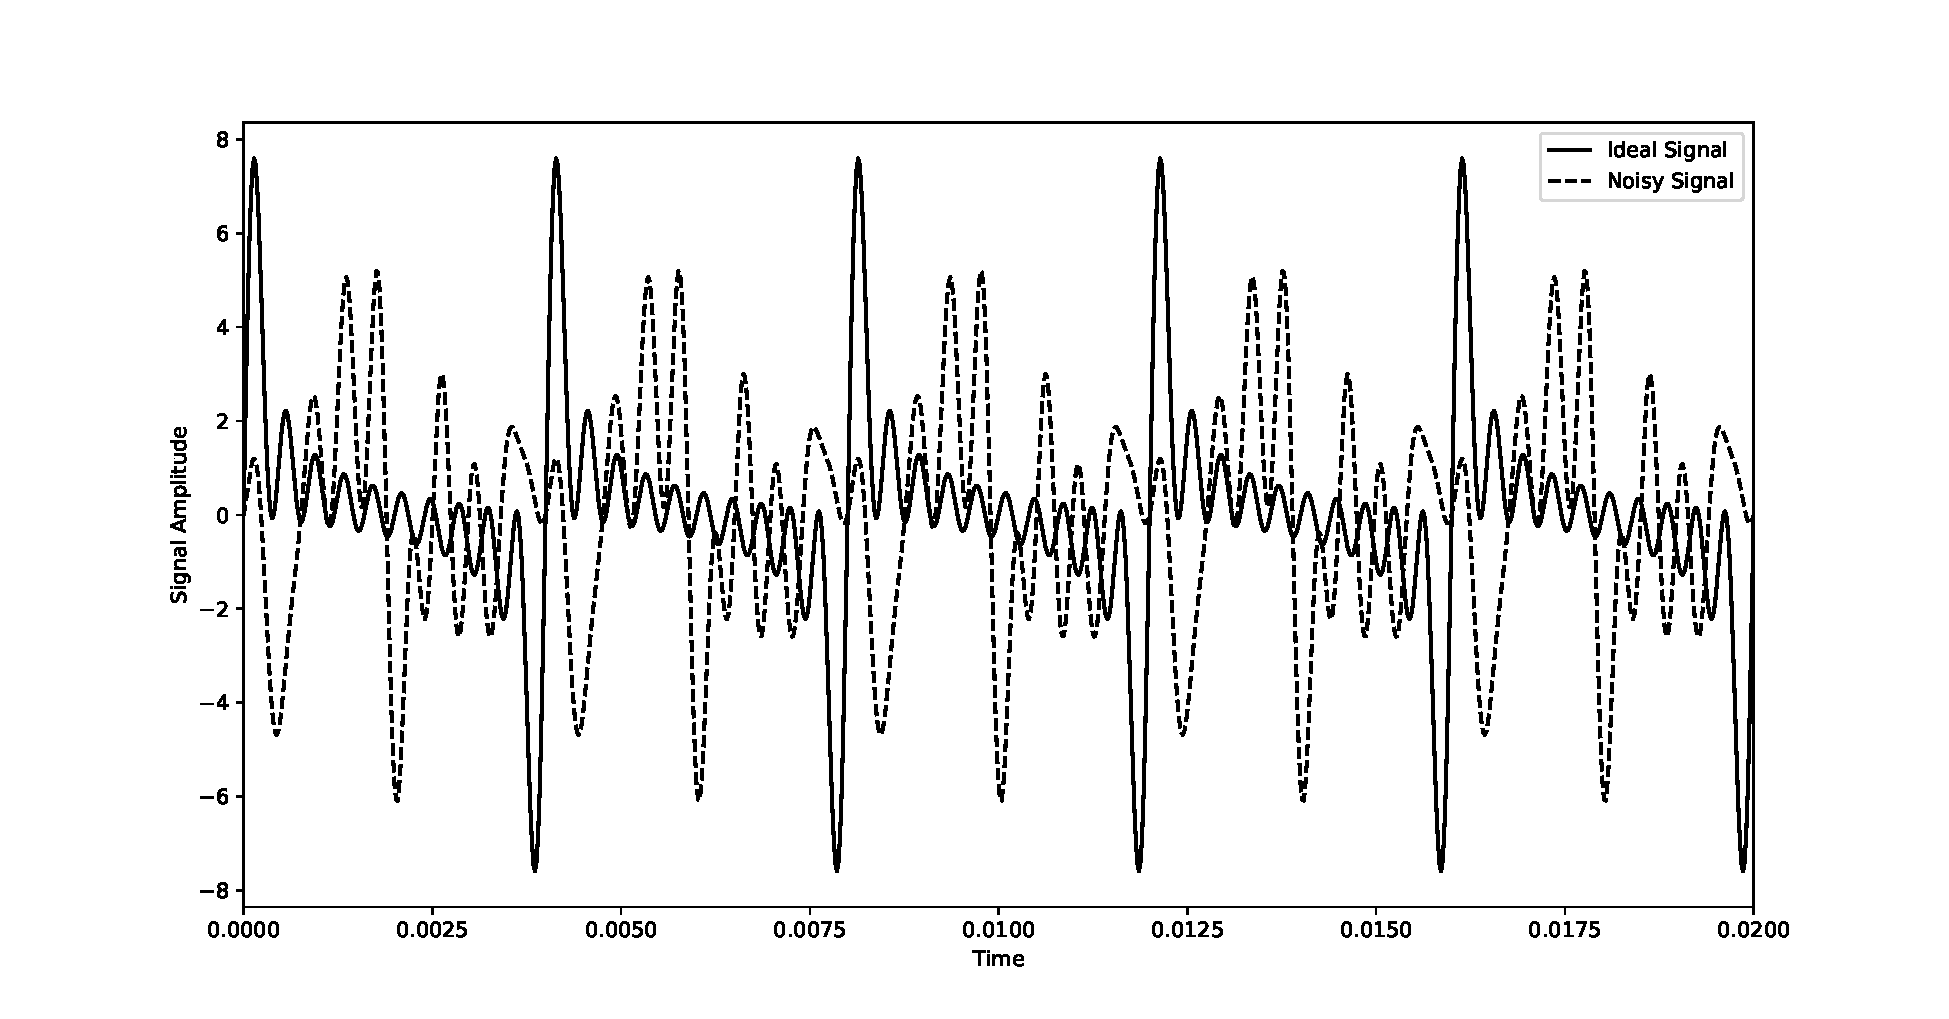
\includegraphics[scale=.3]{Figure_2.pdf}
\footnotetext[2]{\tiny Fredic J. Harris, Chris Dick, $\&$ Michael Rice (2003). Digital Receivers and Transmitters Using Polyphase Filter Banks for Wireless Communications. 
IEEE Transactions On Microwave Theory and Techniques, Vol. 51, No. 4, April 2003, Pg. 1395-1412} 
\end{frame}

\begin{frame}
\frametitle{Signals, Nyquist Theorem, and Frequency Resolution}
\center \textbf{How do we digitize signals?}
\bigskip
\begin{columns}
\column{0.5\textwidth}
Nyquist Theorem
\begin{equation}
f_{crit} = \frac{f_{samp}}{2}
\end{equation}
In radio astronomy, to measure a 10 GHz signal, we would need to process 20 billion samples, or around 160 Gigabytes of data, a second.  Seem unreasonable? It is.
\column{0.5\textwidth}
Along with Nyquist, there is a limit to how much resolution there is between frequencies when using Fast Fourier Transform(FFT), which is given by 
\begin{equation}
f_{res} = f_{samp}/N
\end{equation}
where N is the number of sample points given to the FFT.
\end{columns}
\end{frame}

\begin{frame}
\frametitle{Downsampling: Wait...Which Frequency Was That?}
Since we can't handle all this data, our only recourse is to reduce the sampling rate.  But, this reduces the Nyquist frequency. So, how is this helpful? We need one more friend to help out.
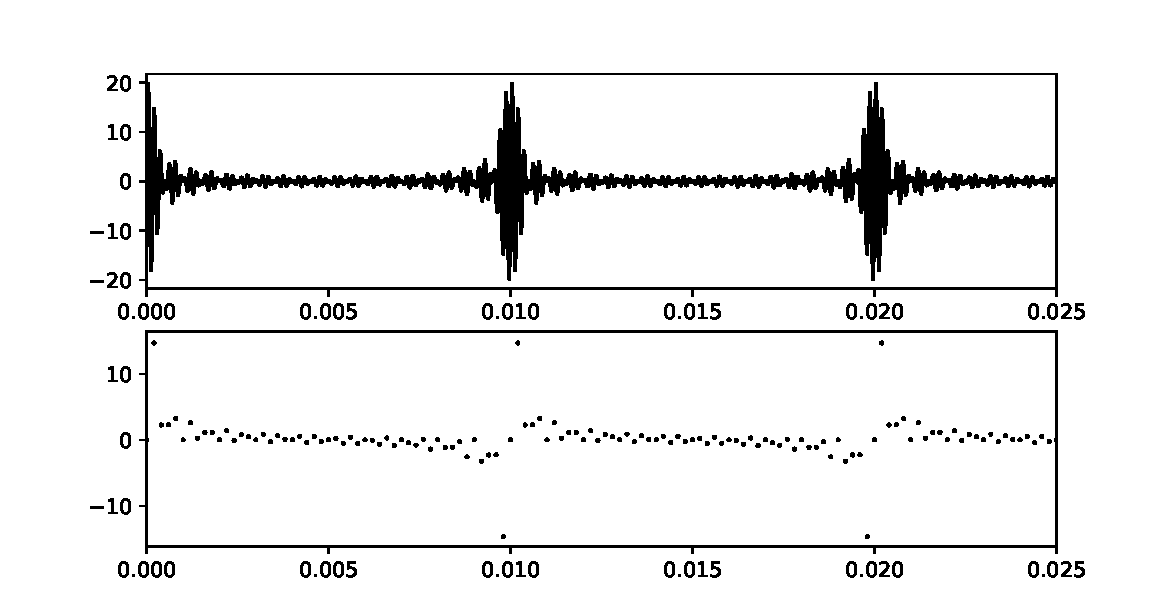
\includegraphics[scale=.55]{Figure_3.pdf}
\end{frame}

\begin{frame}
\frametitle{Downconversion:  The Hero Gotham Deserves}
\center Downconversion allows us to get around the absurd data requirement, while still retaining all of the information contained in the original spectra, but how?

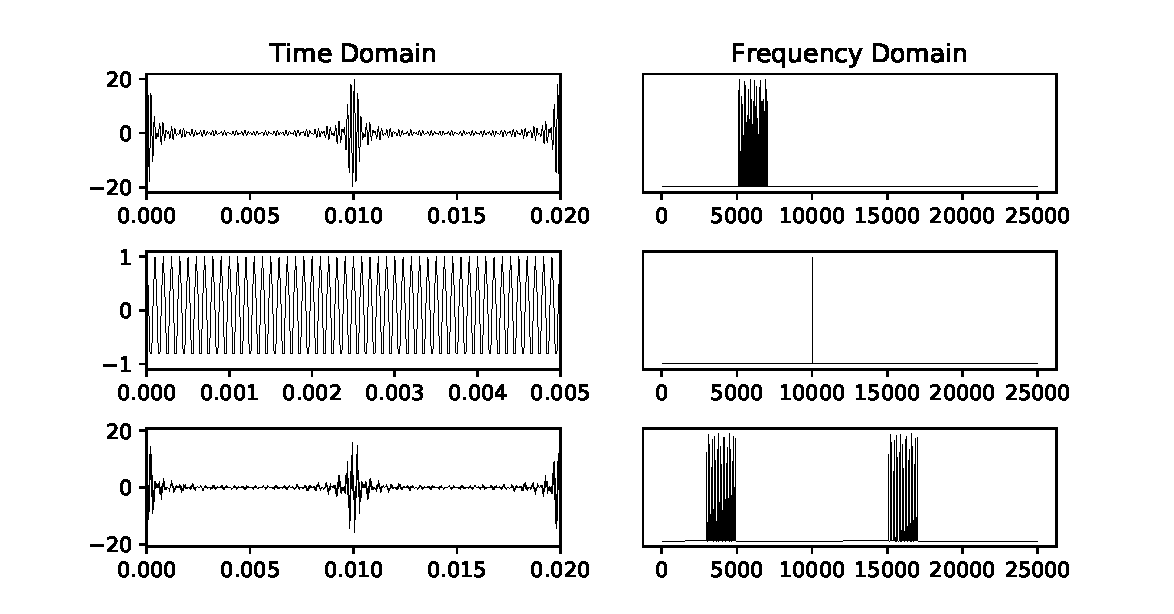
\includegraphics[scale=.58]{Figure_4.pdf}
\end{frame}

\begin{frame}
\frametitle{Downconversion:  The Hero Gotham Deserves}
\center This signal can then be low-pass filtered to a level below a reasonable Nyquist frequency and downsampled. Wait, what's filtering?
\end{frame}

\begin{frame}
\frametitle{Filtering: Finding Needles in Stacks of Needles}
A common technique in digital signal processing(DSP) is the use of digital signal filters, which can lower the power of certain frequency bands while leaving others relatively untouched.  This process is a convolution of the signal with the filter, which is even more expensive.
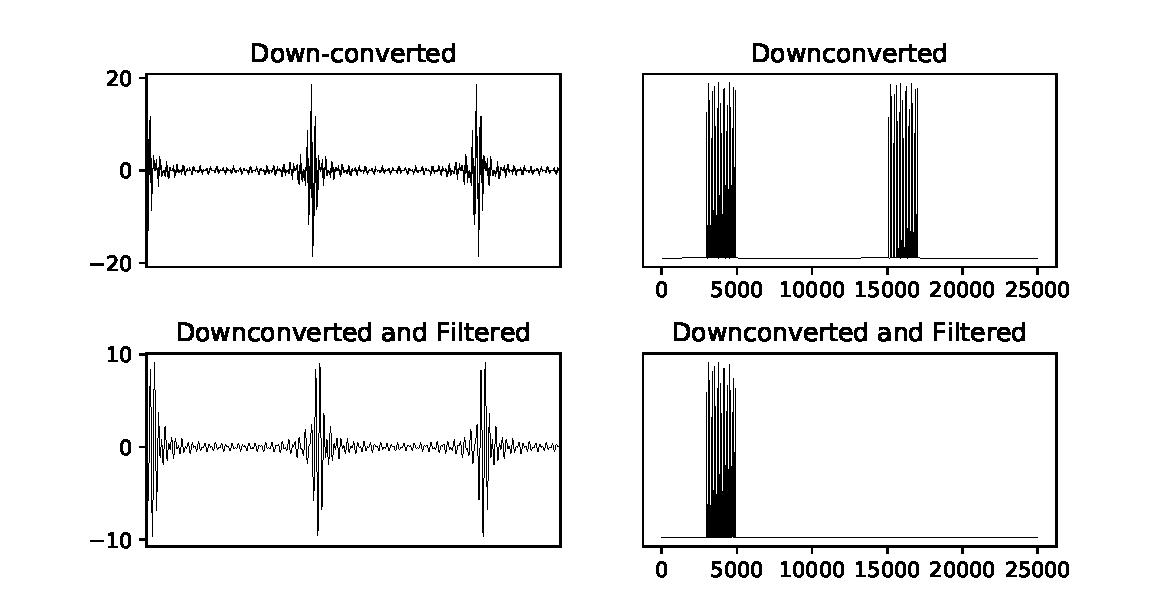
\includegraphics[scale=.58]{Figure_5.pdf}
\end{frame}

\begin{frame}
\frametitle{Wait...This Talk is About Polyphase Filter Banks!}
This is all excellent, but if I don't get to the point Dr. Gary is going to fail me, so....where does the fancy 'Polyphase Filter Bank' phrase fit in? Well, actually, almost everywhere.
\end{frame}

\begin{frame}
\frametitle{Polyphase Filter Banks: Like Split Personalities for Machines}
A filter bank is a method of reconstructing the filter, which was used above, using multiple stages of simpler filters (think 'basis sets').
\end{frame}

\begin{frame}
\frametitle{The Polyphase Implementation: An Example}
For the sake of time, we'll look at how polyphase filtering works mathematically.  Lets start with the definition of the filtered signal,
\begin{equation}
y[n] = \sum_k x[n]h[k-n]
\end{equation}
where y[n] is the filtered signal, x[n] is the raw signal, and h[n] is the filter.
\end{frame}

\begin{frame}
\frametitle{The Polyphase Implementation: An Example}
In a direct computation of the convolution,
$x[n] = \{x_0, x_1, x_2, x_3, x_4, x_5\}$

$h[n] = \{h_0, h_1, h_2, h_3\}$


\begin{center}
  \begin{tabular}{ l|c|c|c|c|c|c|c|r }
    \hline
    $h_0 x_0$ & $h_0 x_1$ & $h_0 x_2$ & $h_0 x_3$ & $h_0 x_4$ & $h_0 x_5$ & & & \\ \hline
    & $h_1 x_0$ & $h_1 x_1$ & $h_1 x_2$ & $h_1 x_3$ & $h_1 x_4$ & $h_1 x_5$ & &\\ \hline
    & &$h_2 x_0$ & $h_2 x_1$ & $h_2 x_2$ & $h_2 x_3$ & $h_2 x_4$ & $h_2 x_5$ &\\ \hline
    & & &$h_3 x_0$ & $h_3 x_1$ & $h_3 x_2$ & $h_3 x_3$ & $h_3 x_4$ & $h_3 x_5$ \\\Xhline{1pt}
    $y_0$ & $y_1$ & $y_2$ & $y_3$ & $y_4$ & $y_5$ & $y_6$ & $y_7$ & $y_8$\\ \hline
  \end{tabular}
\end{center}
\end{frame}

\begin{frame}
\frametitle{The Polyphase Implementation: An Example}
Earlier, we changed the sample rate.  When this happens

\smallskip
  \begin{tabular}{ l|l }
    \hline
    Before Decimation & After Decimation\\ \Xhline{1pt}
	$y_0 = h_0 x_0$ & $y_0 = h_0 x_0$\\ \hline
	$y_1 = h_0 x_1 + h_0 x_1$ & 0\\ \hline 
	$y_2 = h_0 x_2 + h_1 x_1 + h_2 x_0$ & $y_2 = h_0 x_2 + h_1 x_1 + h_2 x_0$\\ \hline 
	$y_3 = h_0 x_3 + h_1 x_2+ h_2 x_2 + h_3 x_1$ & 0 \\ \hline 
	$y_4 = h_0 x_4 + h_1 x_3+ h_2 x_2 + h_3 x_1$ & $y_4 = h_0 x_4 + h_1 x_3+ h_2 x_2 +     	h_3 x_1$\\ \hline
	$y_5 = h_0 x_5 + h_1 x_4 + h_2 x_3 + h_3 x_2$ & 0\\ \hline
	$y_6 = h_1 x_5 + h_2 x_4 + h_3 x_3$ & $y_6 = h_1 x_5 + h_2 x_4 + h_3 x_3$\\ \hline
	$y_7 = h_2 x_5 + h_2 x_4$ & 0\\ \hline
	$y_8 = h_3 x_5$ & $y_8 = h_3 x_5$\\ \hline
  \end{tabular}
  
  \smallskip
  and half of what we have calculated is discarded.  And we worked so hard on it!
\end{frame}

\begin{frame}
\frametitle{The Polyphase Implementation: An Example}
Polyphase Filter Bank Implementation allows us to bypass these extra computations entirely, effectively filtering and downsampling in a single step. For this example, we use an M=2 (2-tap) polyphase filter setup.

\smallskip
\begin{columns}
\column{0.5\textwidth}
  $x[n]^+ = \{x_0, x_2, x_4\}$

  $h[n]^+ = \{h_0, h_2\}$
\begin{center}
  \begin{tabular}{ c|c|c|c }
	\hline
	$h_0 x_0$ & $h_0 x_2$ &$h_0 x_4$\\ \hline
	& $h_2 x_0$ & $h_2 x_2$ &$h_2 x_4$\\ \hline
	$y^+_0$ & $y^+_1$ & $y^+_2$ & $y^+_3$\\ \hline
  \end{tabular}
\end{center}
\column{0.5\textwidth}

$x[n]^- = \{x_1, x_3, x_5\}$

$h[n]^- = \{h_1, h_3\}$
\begin{center}
  \begin{tabular}{ c|c|c|c }
	\hline
	$h_1 x_1$ & $h_1 x_3$ &$h_1 x_5$\\ \hline
	& $h_3 x_1$ & $h_3 x_3$ &$h_3 x_5$\\ \hline
	$y^-_0$ & $y^-_1$ & $y^-_2$ & $y^-_3$\\ \hline
  \end{tabular}
\end{center}
\end{columns}
\end{frame}

\begin{frame}
\frametitle{The Polyphase Implementation: An Example}
Now, we combine the results of these two separate convolutions, but in a unique way.
\smallskip
\begin{center}
  \begin{tabular}{l}
    \hline
    Convolution and Decimation\\ \Xhline{1pt}
	$y^+_0 + y^-_{-1}= h_0 x_0 = \mathbf{y_0}$\\ \hline
	$y^+_1 + y^-_0 = h_0 x_2 + h_1 x_1 + h_2 x_0 = \mathbf{y_2}$\\ \hline 
	$y^+_2 + y^-_1 = h_0 x_4 + h_1 x_3+h_2 x_2 + h_3 x_1 = \mathbf{y_4}$\\ \hline
	$y^+_3 + y^-_2 = h_1 x_5 + h_2 x_4 + h_3 x_3 = \mathbf{y_6}$\\ \hline
	$y^+_4 + y^-_3 = h_3 x_5 = \mathbf{y_8}$\\ \hline
  \end{tabular}
\end{center}  
and we have accomplished the same convolution, but now the unnecessary calculations are not used.

\end{frame}

\begin{frame}
\frametitle{Wrapping It Up}
Here I gave an example of how to use a polyphase filter bank to lowpass and decimate a signal. Combined with an array of reference oscillators, this becomes an incredibly efficient channelizer.  One powerful feature we didn't discuss was its effect on Gibbs ringing (side lobes). 

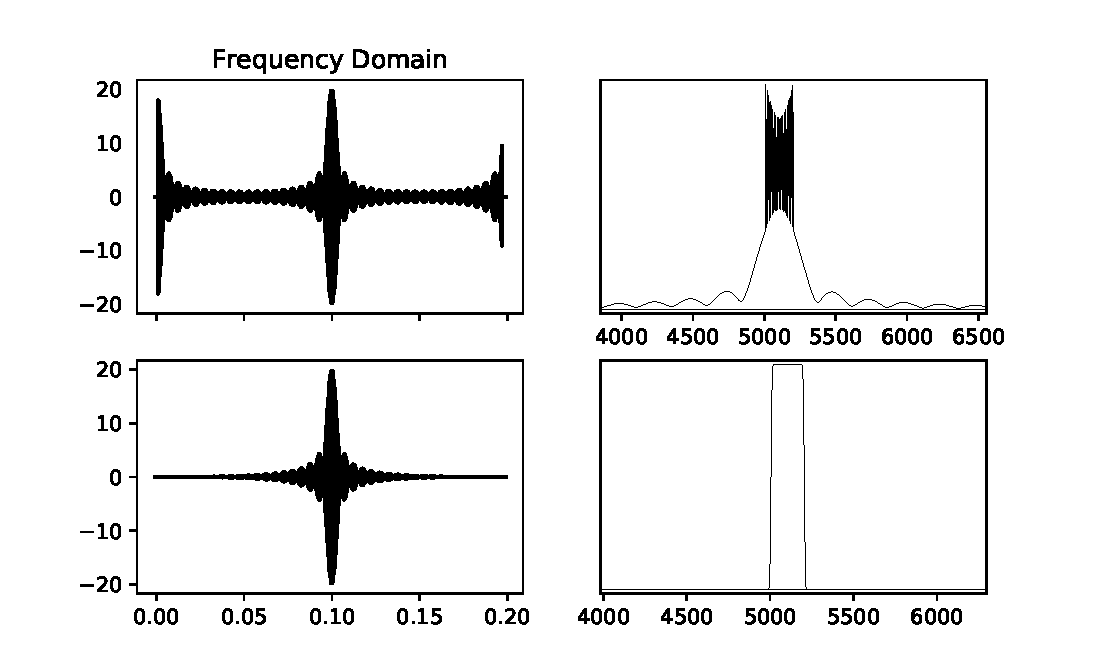
\includegraphics[scale=.55]{Figure_6.pdf}
\end{frame}

\begin{frame}

\frametitle{But Don't Windows Do That?}
It is quite common to multiply a signal by a windowing function before feeding it to an FFT in order to minimize the presence of side lobes in the spectra.  This comes at the price of frequency resolution.


\end{frame}
\begin{frame}
\frametitle{The End}
\center
\huge Thanks For Your Attention. 
\end{frame}
\end{document}

